\documentclass{article}
\usepackage{amsmath}
\usepackage{amssymb}
\usepackage{array}
\usepackage{booktabs}
\usepackage{makecell}
\usepackage{multirow}
\usepackage{enumitem}
\usepackage{diagbox}
\usepackage{tabularx}
\usepackage{graphicx}
% \usepackage[top=3cm,bottom=2cm,left=2cm,right=2cm]{geometry} % 页边距
\title{Software System Design-Architecture\\Assignment 3\\C4 System Architecture Design}
\author{4 people}

\begin{document}
	\maketitle
	\newpage
	\section{Deploying ADD method in C4 Design}
	\subsection{Important Non-functional Requirements}
	The important non-functional requirements we identified are listed bellow:\\
	...
	\subsection{Records of ADD iterations}
	

	\section{Final Software Architecture Documentation}
	\subsection{Documentation Roadmap}
	\subsubsection{Scope and summary}
	This documentation is built for presence, explanation and analysis of the architecture of Call Center Customer Care(C4) System, which will be employed by ** US telecommunication company. In this documentation, expression and illustration of modules and theirs relationship will be covered, but not all functions of the system are included.
	\subsubsection{How the documentation is organized}
	cateloge
	\subsubsection{View overview}
	4 Views are employed to illustrate the architecture, including:\\  
	Decomposition view: The elements of this view are static modules, and connections illustrate their relationship.\\  
	Shared-data view: We using this view to express how important data are shared and protected from inconsistency resulted by business events....  \\
	Deployment view: This view also illustrate different parts of the software. Distinguished with module view, it focuses on the runtime status rather than the static status of the system.\\
	All of the three views are following the standard UML specification.
	\subsubsection{How stakeholders can use this documentation}
	Use for specification, evaluation, development, test, deployment.

	\subsection{How a View Is Documented}
	Refer to the view template

	\subsection{System Overview}
	System functions, users, important background, constrains.
	
	\subsection{Views}

		\subsubsection{Shared-Data View} 
			\paragraph{Section 1: The Primary Presentation}
			\begin{center}
			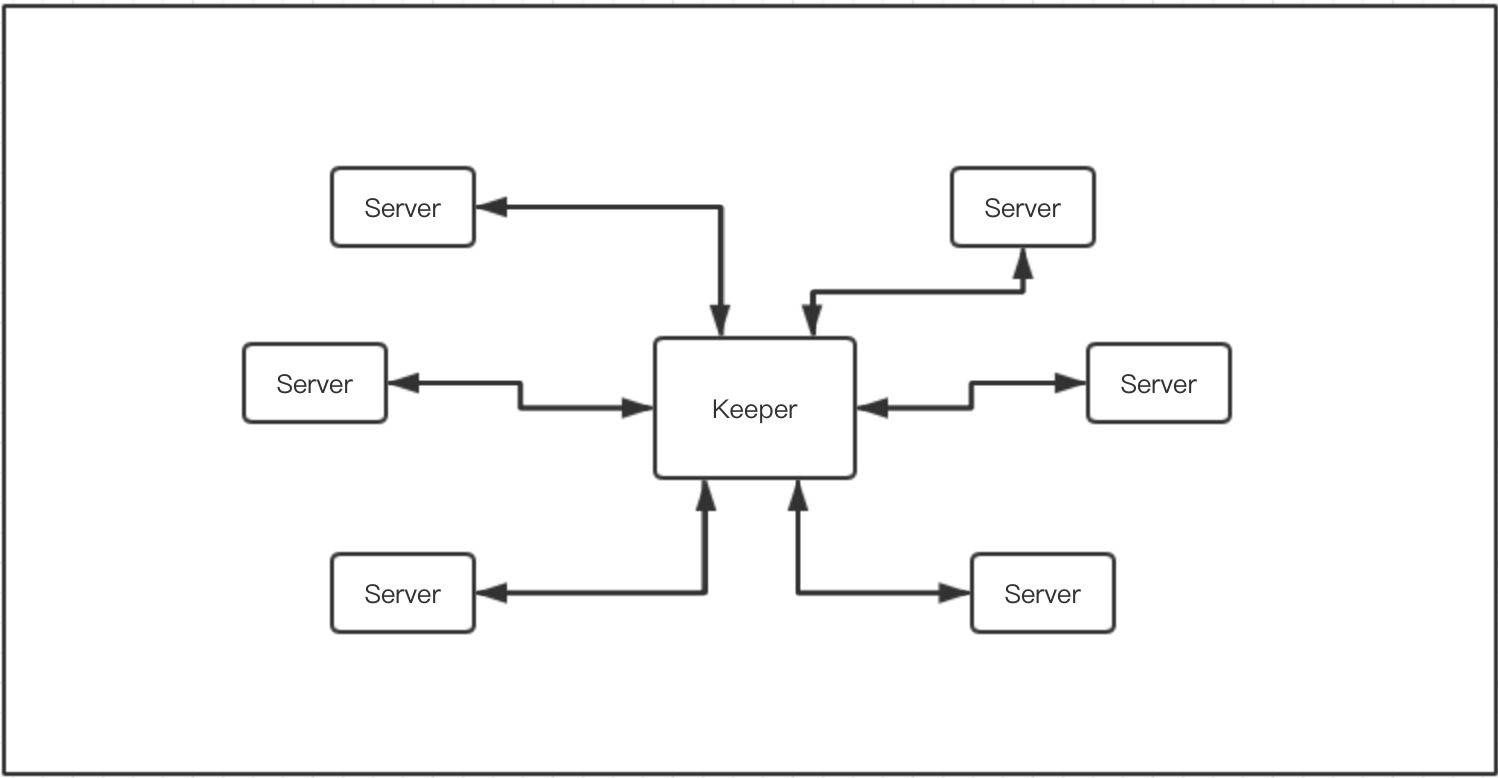
\includegraphics[scale=0.3]{share.png}
			\end{center}
			\paragraph{Section 2: The Element Catalog}
			\subparagraph{Elements and their properties}
			\begin{itemize}
			\item{Keeper} The keeper is a data storage center which holds the shared data.
			\item{Server} The server is an entity which stores and fetches data from the Keeper. For example, when a customer temporarily terminates the process, server should save the context for a future reference.
			\end{itemize}
			\subparagraph{Relations and their properties}
			During the fetching process, there may not exist the record, so there should be an exception. Also, in the saving process, to those records that already existed, saving process should be an update to the old version.
			\subparagraph{Element interfaces}
			The Keeper should provide the find and insert interfaces to the servers.
			\subparagraph{Element behavior}
			The servers save and fetch the data from the Keeper.
			\paragraph{Section 3: Context Diagram}
			\begin{center}
			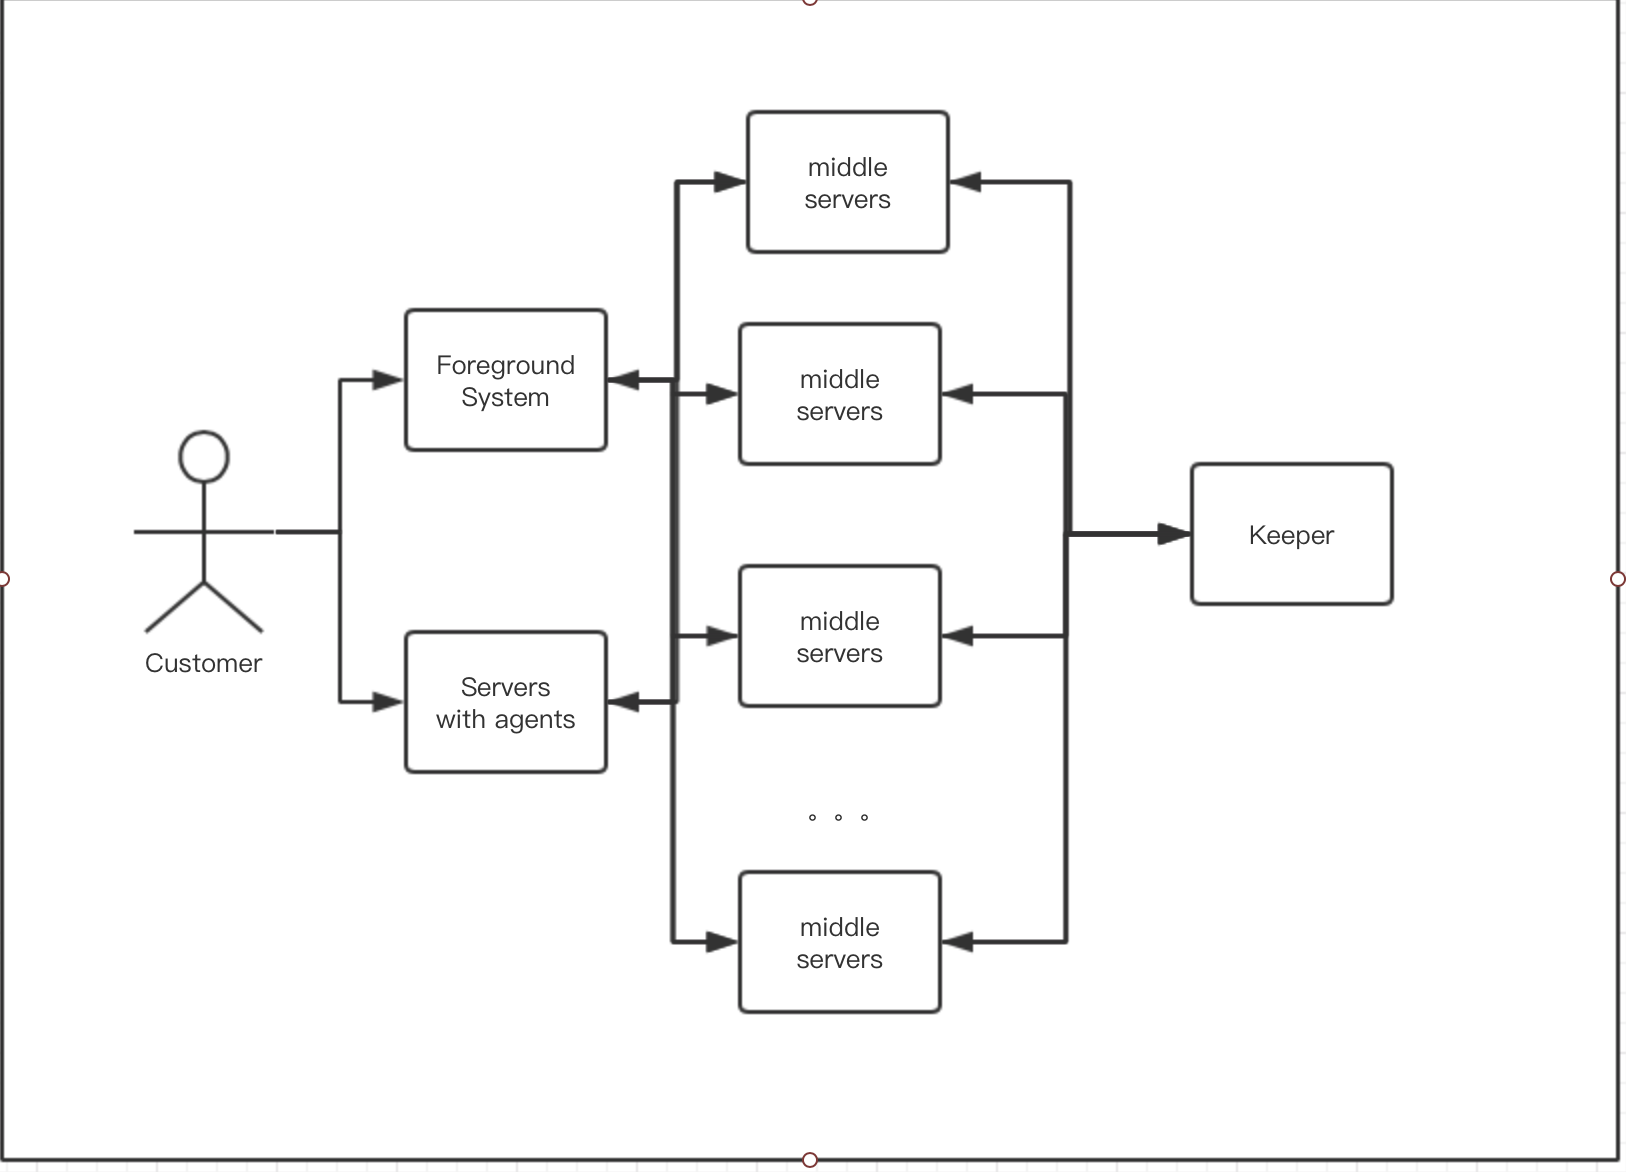
\includegraphics[scale=0.3]{share2.png}
			\end{center}
			\paragraph{Section 4: Variability Guide}
			Because the data storage is not the only responsibility keeper takes, so in the future, it may be  divided into several more specific components, that is to say, the keeper in this view may be changed to a data repository or other data center.
			\paragraph{Section 5: Rationale}
			The design problem came from the requirement "A customer can be interrupted (for technical reasons, for example) or suspended by the customer or the representative ... In any case, C4 has to manage the context that persists and can be recalled."
			In order to do this, there should be a mechanism that stores and fetches the context. There are several options. For example, we can save the information in the agent's PC, or save in the DB provided by the third party. But both of them are infeasible. There is no persistent data caching on the agent workstations, and DB may not be changed since it is provided by the third party. So finally, we choose to save the information in the Keeper, as it is also used to synchronize the event and resolve the conflict as mentioned in the sections before.

	\subsection{Mapping Between Views}
	TODO

	\subsection{Rationale}
	Explain what decision we have made in our views.

	\subsection{Directory}


	\section{Personal Remarks}
	\subsection{Statement of ...}
	\subsection{Statement of ...}
	\subsection{Statement of ...}
	\subsection{Statement of ...}
\end{document}